% Standalone source for ISR correction-step flow diagram.
% Build: make figures/isr-pipeline.pdf
% (Or: cd figures/src && pdflatex -interaction=nonstopmode -halt-on-error -jobname=isr-pipeline -output-directory=.. to-make-isr-pipeline.tex)
\documentclass[tikz, border=4pt]{standalone}
\usetikzlibrary{positioning, arrows.meta, calc, fit, backgrounds}

\definecolor{staticfill}{HTML}{EAF2FB}
\definecolor{staticline}{HTML}{6495ED}
\definecolor{dynamicfill}{HTML}{FCEFE0}
\definecolor{dynamicline}{HTML}{C77F2B}
\definecolor{inputfill}{HTML}{FFFFFF}
\definecolor{inputline}{HTML}{ECECEC}

% Keep labels clean: no automatic hyphenation inside boxes.
\hyphenpenalty=10000
\exhyphenpenalty=10000
\hbadness=10000

\tikzset{
  base/.style={
    draw,
    rounded corners=5.0pt,
    align=center,
    font=\scriptsize,  % small
    text width=2.05cm, % 3.05
    minimum height=3.0em,
    inner xsep=4pt,
    inner ysep=3pt,
    line width=1.0pt,  % 0.6pt
  },
  static/.style={base, fill=staticfill, draw=staticline},
  dynamic/.style={base, fill=dynamicfill, draw=dynamicline},
  input/.style={base, fill=inputfill, draw=inputline},
  optional/.style={base, fill=staticfill, draw=staticline, dash pattern=on 3pt off 2pt},
  % arr/.style={
  %   -{Stealth[length=5pt, width=4pt]},
  %   line width=0.7pt,
  %   draw=black!65,
  %   rounded corners=3pt,
  % },
  arr/.style={-{>[length=15pt, width=50pt, angle=60:5pt]}, lightgray, line width=0.75pt},
  stepnum/.style={
    font=\scriptsize,
    anchor=north west,
    inner sep=0pt,
  },
}

% #1 = node options, #2 = name, #3 = step number, #4 = label text (use \\ between lines)
\newcommand{\stepnode}[4][]{%
  \node[#1, minimum height=3.0em, label={[stepnum, xshift=4pt, yshift=-3pt]north west:#3}] (#2) {%
    \vspace{0.7em}\shortstack[c]{#4}%
  }%
}

\begin{document}
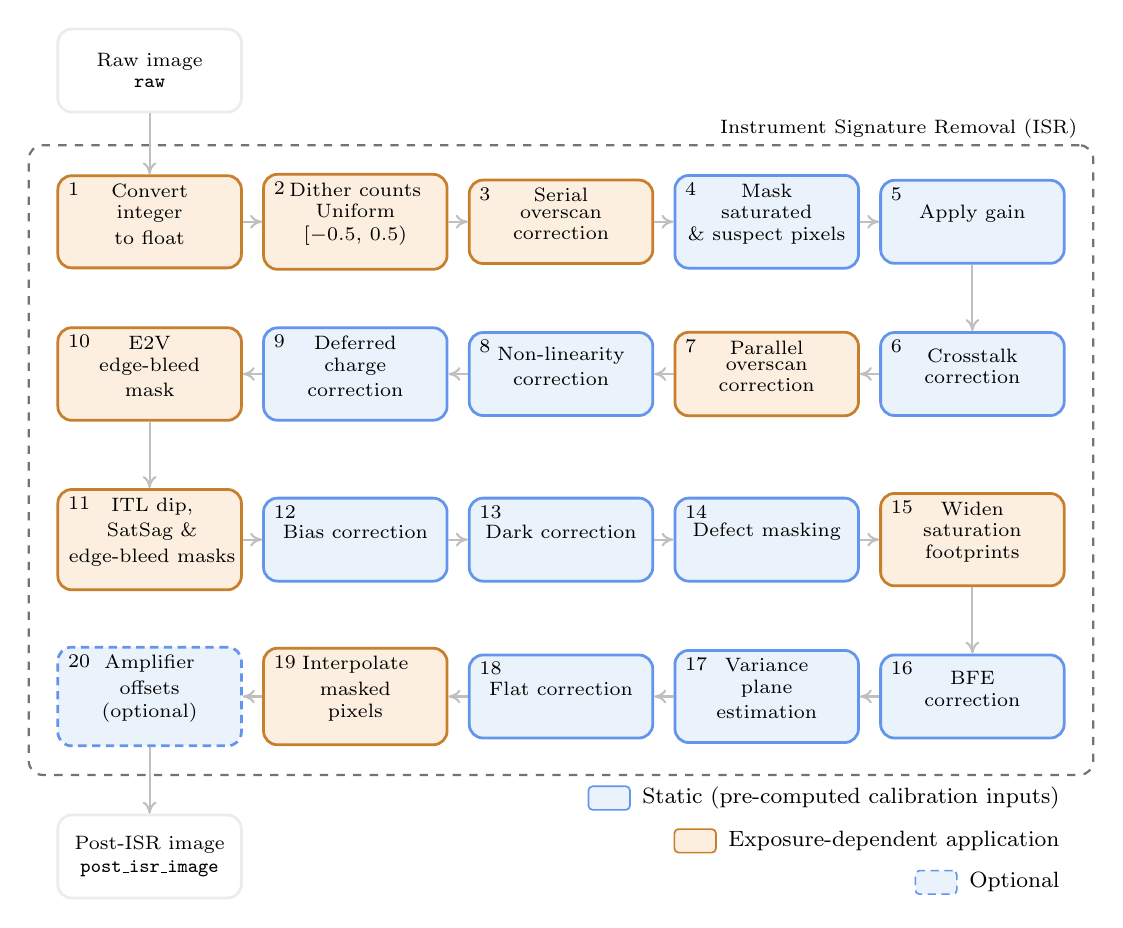
\begin{tikzpicture}

% Lead-in
\node[input] (raw) {\shortstack[c]{Raw image\\\texttt{raw}}};

% Row 1 (left to right): steps 1--5
\stepnode[dynamic, below=2.2em of raw]{n01}{1}{Convert\\integer\\to float};
\stepnode[dynamic, right=0.7em of n01]{n02}{2}{Dither counts\\Uniform\\$[-0.5,\,0.5)$};
\stepnode[dynamic, right=0.7em of n02]{n03}{3}{Serial\\overscan\\correction};
\stepnode[static, right=0.7em of n03]{n04}{4}{Mask\\saturated\\\& suspect pixels};
\stepnode[static, right=0.7em of n04]{n05}{5}{Apply gain};

% Row 2 (right to left): steps 6--10
\stepnode[static, below=2.4em of n05]{n06}{6}{Crosstalk\\correction};
\stepnode[dynamic, left=0.7em of n06]{n07}{7}{Parallel\\overscan\\correction};
\stepnode[static, left=0.7em of n07]{n08}{8}{Non-linearity\\correction};
\stepnode[static, left=0.7em of n08]{n09}{9}{Deferred\\charge\\correction};
\stepnode[dynamic, left=0.7em of n09]{n10}{10}{E2V\\edge-bleed\\mask};

% Row 3 (left to right): steps 11--15
\stepnode[dynamic, below=2.4em of n10]{n11}{11}{ITL dip,\\SatSag \&\\edge-bleed masks};
\stepnode[static, right=0.7em of n11]{n12}{12}{Bias correction};
\stepnode[static, right=0.7em of n12]{n13}{13}{Dark correction};
\stepnode[static, right=0.7em of n13]{n14}{14}{Defect masking};
\stepnode[dynamic, right=0.7em of n14]{n15}{15}{Widen\\saturation\\footprints};

% Row 4 (right to left): steps 16--20
\stepnode[static, below=2.4em of n15]{n16}{16}{BFE\\correction};
\stepnode[static, left=0.7em of n16]{n17}{17}{Variance\\plane\\estimation};
\stepnode[static, left=0.7em of n17]{n18}{18}{Flat correction};
\stepnode[dynamic, left=0.7em of n18]{n19}{19}{Interpolate\\masked\\pixels};
\stepnode[optional, left=0.7em of n19]{n20}{20}{Amplifier\\offsets\\(optional)};

% Row 5 (left to right):
\node[input, below=2.4em of n20]   (n21) {\shortstack[c]{Post-ISR image\\\texttt{post\_isr\_image}}};

% Dashed frame around ISR steps only (excludes raw input and post-ISR output).
\begin{scope}[on background layer]
  \node[
    dashed,
    draw=black!55,
    line width=0.8pt,
    rounded corners=5pt,
    inner sep=10pt,
    fit=(n01)(n02)(n03)(n04)(n05)(n06)(n07)(n08)(n09)(n10)(n11)(n12)(n13)(n14)(n15)(n16)(n17)(n18)(n19)(n20),
  ] (isrframe) {};
\end{scope}
\node[
  anchor=south east,
  font=\scriptsize,
  inner sep=0pt,
] at ([xshift=-6pt, yshift=+2pt]isrframe.north east) {Instrument Signature Removal (ISR)};

% --- Flow arrows -------------------------------------------------------
\draw[arr] (raw.south) -- (n01.north);
% Row 1 (L->R)
\foreach \a/\b in {n01/n02, n02/n03, n03/n04, n04/n05}
  {\draw[arr] (\a.east) -- (\b.west);}
\draw[arr] (n05.south) -- (n06.north);     % turn 1->2
% Row 2 (R->L)
\foreach \a/\b in {n06/n07, n07/n08, n08/n09, n09/n10}
  {\draw[arr] (\a.west) -- (\b.east);}
\draw[arr] (n10.south) -- (n11.north);     % turn 2->3
% Row 3 (L->R)
\foreach \a/\b in {n11/n12, n12/n13, n13/n14, n14/n15}
  {\draw[arr] (\a.east) -- (\b.west);}
\draw[arr] (n15.south) -- (n16.north);     % turn 3->4
% Row 4 (R->L)
\foreach \a/\b in {n16/n17, n17/n18, n18/n19, n19/n20}
  {\draw[arr] (\a.west) -- (\b.east);}
% Row 5
\draw[arr] (n20.south) -- (n21.north);

% --- Legend (bottom right, 3 rows, right-aligned) ----------------------
\begin{scope}[
  swatch/.style={draw, rounded corners=1.5pt, minimum width=1.5em, minimum height=0.85em, inner sep=0pt, line width=0.6pt},
  lbl/.style={font=\footnotesize, inner sep=2pt},
]
  \coordinate (legbr) at ($(n16.south east)+(0,-1.5em)$);
  \node[lbl, anchor=north east] (l1) at (legbr) {Static (pre-computed calibration inputs)};
  \node[swatch, fill=staticfill, draw=staticline, anchor=east, left=2pt of l1.west] (s1) {};
  \coordinate (l2pos) at ($(l1.south east)+(0,-0.35em)$);
  \node[lbl, anchor=north east] (l2) at (l1.east |- l2pos) {Exposure-dependent application};
  \node[swatch, fill=dynamicfill, draw=dynamicline, anchor=east, left=2pt of l2.west] (s2) {};
  \coordinate (l3pos) at ($(l2.south east)+(0,-0.35em)$);
  \node[lbl, anchor=north east] (l3) at (l1.east |- l3pos) {Optional};
  \node[swatch, fill=staticfill, draw=staticline, dash pattern=on 3pt off 2pt, anchor=east, left=2pt of l3.west] (s3) {};
\end{scope}

\end{tikzpicture}
\end{document}
